\documentclass{article}
\usepackage{graphicx}
\usepackage{amsmath}
\usepackage[mathletters]{ucs}
\usepackage[utf8x]{inputenc}
\usepackage{listings}
\lstnewenvironment{code}{\lstset{language=Haskell,basicstyle=\small\ttfamily}}{}

\setlength{\parindent}{0pt}
\setlength{\parskip}{6pt plus 2pt minus 1pt}

\usepackage{pgf, tikz}
\usetikzlibrary{shapes}
\usetikzlibrary{shapes.multipart}
\usetikzlibrary{arrows}

\lstdefinelanguage{FSharp}
      {morekeywords={let, new, match, inherit, abstract, with, rec,
          open, module, namespace, type, of, member, and, for, in, do,
          begin, end, fun, function, try, mutable, if, then, else,
          class, interface, end},
    keywordstyle=\color{blue},
    basicstyle = \small,
    sensitive=false,
    morecomment=[l][\color{green!50!black!80}]{///},
    morecomment=[l][\color{green!50!black!80}]{//},
    morecomment=[s][\color{green!50!black!80}]{{(*}{*)}},
    morestring=[b]",
    stringstyle=\color{red},
    columns=fullflexible
    }


\lstdefinelanguage{Smalltalk}{
  basicstyle=\ttfamily,
  keywordstyle=\bfseries,
  morekeywords={self,super,true,false,nil,thisContext}, % This is overkill
  morestring=[d]',
  morecomment=[s]{"}{"},
  alsoletter={\#:},
  escapechar={!},
}[keywords,comments,strings]


\newcommand{\Blue}[1]{\color{blue}#1\color{black}\xspace}


\usepackage{array}
% This is needed because raggedright in table elements redefines \\:
\newcommand{\PreserveBackslash}[1]{\let\temp=\\#1\let\\=\temp}
\let\PBS=\PreserveBackslash

%%%%%%%%%%%%%% 
\newcommand{\solution}[1] {}
%\newcommand{\solution}[1] {\textbf{Solutions:}\\ #1}

%\newcommand{\comment}[1]{}
\newcommand{\comment}[1]{\marginpar{#1}}


\begin{document}
\newcommand{\examtime}{14:00, Wednesday December 15th, 2010}
\newcommand{\points}[1]{\marginpar{\bf #1 points}}
\noindent
\begin{tabular}{lr}
CHALMERS TEKNISKA H\"OGSKOLA &\examtime{}.\\
Dept. of Computer Science and Engineering & Programming Paradigms\\
John Hughes                  & DAT120 / DIT330(GU) \\
\end{tabular}

\vspace{2.5cm} \noindent
\begin{center} {\LARGE
Exam in Programming Paradigms}
\end{center}

\vspace{1.5cm}

\noindent
\examtime{}.\\
\begin{tabular}{lllc}
\textbf{Lecturer:} &  John Hughes  & tel 070 756 3760 & (Examinator)\\
\textbf{Lecturer:} & Richard Bubel & tel 073 965 7355 & \\ 
\end{tabular}
\vspace{1cm}

\noindent
Permitted aids:\\
English-Swedish or English-other language dictionary.

There are 6 questions on 13 numbered pages. 

Five of the six questions are ordinary questions: One on functional
programming (12 points), one on concurrency oriented programming (12
points), one on basic imperative and object-oriented concepts (10
points), one on object-oriented programming (15 points) and one on
logic programming (12 points).

The sixth and last question is a bonus question on the guest lecture,
worth 1 point. The total sum is 62 points.


\textbf{Chalmers:}
24 points is required to pass (grade 3), 36 points is required for
grade 4, and 48 points is required for grade 5. 

\textbf{GU:}
24 points is required to pass (grade G) and 48 points is required for
grade VG.


\newpage 
\hfill\\
\newpage

\section{Functional Programming [12 points]}

\begin{enumerate}

\newcommand{\id}[1]{\mbox{\it #1}}

\item Given that
\begin{eqnarray*}
\id{twice} &=& \lambda f.\lambda x.f~(f~x)
\end{eqnarray*}
show how to simplify 
\[ \id{twice}~\id{twice}~f~x \]
as far as possible using $\beta$-reductions.  Apply $\beta$-reductions
one at a time, and write out the result of each step explicitly.
\points{2}

\item 
Study the following Haskell definition of the list append function:
\begin{verbatim}
[]     ++ ys = ys
(x:xs) ++ ys = x : (xs ++ ys)
\end{verbatim}
List structures can be drawn diagrammatically using boxes to represent
{\em cons} cells and arrows to represent pointers\dots for example, if
\verb!xs! is the list \verb![1,2]! and \verb!ys! is the list
\verb![3,4]!, then the heap containing these two lists can be drawn
as:
\begin{center}
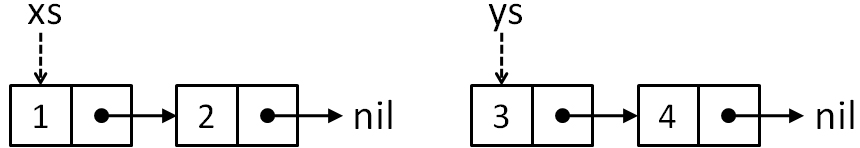
\includegraphics[width=7cm]{Lists.jpg}
\end{center}
{\em Copy this diagram}, and add to your drawing the list \verb!zs! defined by
\begin{verbatim}
zs = xs ++ ys
\end{verbatim}
Make sure that any sharing in the heap is shown accurately in your diagram.
\points{1}

\item
Study the following Haskell definitions, of the list reverse function
and a mysterious function:
\begin{verbatim}
reverse []     = []
reverse (x:xs) = reverse xs ++ [x]

mystery xs []     = xs
mystery xs (y:ys) = mystery (y:xs) ys
\end{verbatim}
In the following parts, assume that \verb!as! is a list of $m$
elements, and \verb!bs! is a list of $n$ elements.
\begin{enumerate}
\item
How many new cons cells are allocated during the evaluation of
\verb!as ++ bs!?
\points{1}
\item
How many cons cells are
allocated during the evaluation of \verb!reverse as!?
\points{1}
\item
How many cons cells are allocated during the evaluation of
\verb!mystery as bs!?
\points{1}
\item
What well-known compiler optimization is applicable to \verb!mystery!,
but not to \verb!reverse!?
\points{1}

\end{enumerate}
\item
QuickCheck properties take the form of boolean functions whose result
should always be true. For example,
\begin{verbatim}
prop_reverse xs =
  twice reverse xs == xs
\end{verbatim}
\begin{enumerate}
\item
What is the value of \verb!mystery [1,2] [3,4]!?
\points{1}
\item
Propose a QuickCheck property relating \verb!mystery!, \verb!reverse!
and \verb!(++)!.
\points{1}
\item
Give a more efficient definition of the \verb!reverse! function than
the one above, making use of \verb!mystery! in the definition.
\points{1}
\end{enumerate}

\item
The Haskell standard {\em higher-order function} \verb!foldl! is defined by
\begin{verbatim}
foldl f z []     = z
foldl f z (x:xs) = foldl f (f z x) xs
\end{verbatim}
Compare the definitions of \verb!foldl! and \verb!mystery!, and give
an alternative definition of \verb!mystery! in the form
\begin{verbatim}
mystery xs ys = foldl ...
\end{verbatim}
\points{2}

\end{enumerate}



\newpage
\section{Concurrency Oriented Programming [12 points]}

\begin{enumerate}
\item
How are Erlang data structures protected against simultaneous
modification by concurrent processes?
\points{1}

\item
Study the following code, which starts a server managing an integer value:
\begin{verbatim}
server() ->
    spawn(fun() -> server(0) end).

server(N) ->
    receive
        {read,Pid} ->
            Pid ! {self(),N},
            server(N);
        {write,New} ->
            server(New)
    end.
\end{verbatim}
Write the following functions for use in clients of the server:
\begin{enumerate}
\item
\verb!read(ServerPid)!, which returns the value \verb!N! currently managed by the server,
\points{1}
\item
\verb!write(ServerPid,New)!, which updates the value currently managed by the server to \verb!New!.
\points{1}
\end{enumerate}

\item
What value(s) can the following function return:
\begin{verbatim}
test() ->
    Server = server(),
    spawn(fun() -> write(Server,read(Server)+1) end),
    spawn(fun() -> write(Server,read(Server)+1) end),
    read(Server).
\end{verbatim}
\points{1}

\item
Extend the server to handle two new requests, to {\em lock} and {\em
  unlock} the server, such that the next request serviced after a {\em
  lock} must be an {\em unlock} request from the same client. Define
the following functions for use in clients:
\begin{enumerate}
\item
\verb!lock(ServerPid)!, which returns the value \verb!N! currently
managed by the server, and prevents any other request from being
serviced until
\points{1}
\item
\verb!unlock(ServerPid,New)!, which updates the value currently
managed by the server to \verb!New!, and permits other clients to use
the server again.
\points{1}
\end{enumerate}
Write the code which must be added to the \verb!server(N)! function to
handle these two new requests.
\points{2}
\item
What happens to requests sent to the server while it is locked by
another client?
\points{1}
\item
What happens (to the server and other clients) if a client crashes
after calling \verb!lock(Server)!, but before calling
\verb!unlock(Server,New)!?
\points{1}
\item
What is the effect of calling \verb!link(Pid)! in an Erlang process?
\points{1}
\item
How would you make the server {\em fault-tolerant}, so that if a
client crashes while holding the lock, then the server and other
clients are unaffected?  Show the code that you would add to the
\verb!server(N)! function.  \points{1}


\end{enumerate}


\newpage




\newpage

\section{Basic Imperative and Object-Oriented Concepts [10 points]}

\begin{center}
\begin{lstlisting}[language=Java, title=- Listing 3.1 - , columns=flexible, basicstyle=\small]
void f(int x by-??, int y by-??) {
   x = x * y;
   y = (x - y) + 5;
}

void m() {
  int a; int b;
  a = 3;
  b = a;  (*)
  f(a, b); (**)
  ...
}
\end{lstlisting}
\end{center}

\begin{enumerate}
\item \comment{\textbf{3 points}} Assume the assignment at (*) in
  Listing 3.1 uses
  \emph{copy semantics}. Give the values of \texttt{a} and \texttt{b}
  at (**) directly after the call to \texttt{f} returned if
  \begin{enumerate}
  \item both parameters are passed by-value.
  \item both parameters are passed by-reference.
  \item the first parameter \texttt{x} is passed by-value and the
    second parameter \texttt{y} is passed by-value-result.
  \end{enumerate} 
\item \comment{\textbf{3 points}} Assume now that the assignment at
  (*) in Listing 3.1 uses \emph{reference semantics}. Like in the
  previous assignment, give the values of \texttt{a} and \texttt{b} at
  (**) directly after the call to \texttt{f} returned if
  \begin{enumerate}
  \item both parameters are passed by-value.
  \item both parameters are passed by-reference.
  \item the first parameter \texttt{x} is passed by-value and the
    second parameter \texttt{y} is passed by-value-result. 
  \end{enumerate} 
\item \comment{\textbf{2 points}} Let $sp$ denote the base
  address/stack pointer for an activation record. Access to e.g. local
  variables is the computed by an offset $sp+\mathit{offset}$. Assume
  that array-typed parameters are passed by-value and stored
  completely within an activation record. Where should the arrays be
  stored in the activation record: at the beginning or at the end? Why?
  (one sentence) \newpage
\item \comment{\textbf{2 points}} Consider the following program:
\begin{lstlisting}[language=Java, columns=flexible]
int f (int x, int y) {
  if (y == 0) { 
     return x; (*) 
  } else {
     return f(y, x%y);
  }
}
\end{lstlisting}
Consider the call 
\begin{center}
  \lstinline[language=Java, columns=flexible]{f(4,2)} 
\end{center}
Give the number of activation records on the stack resulting from the
above call just before returning from the base case (*), i.e.,
directly after assigning the return value, but before popping the last
activation record from the stack. Give also the activation record on
top of the stack (the last allocated one). Name all slots/components
of the activation record and their content explicitly.
\end{enumerate}

\solution{
\begin{enumerate}
  \item \hfill \\
  \begin{tabular}{cc}
    a & b \\ \hline
    3 & 3 \\
    9 & 11\\
    3 & 11     
  \end{tabular}

  \item \hfill \\
  \begin{tabular}{cc}
    a & b \\ \hline
    3 & 3 \\
    5 & 5\\
    11 & 11 \\     
  \end{tabular}
\item Arrays should be allocated at the end. This allows the other
  (fixed-sized) parameters to be accessed easy and fast. 
\item Number of activation records on stack $2$.\\

  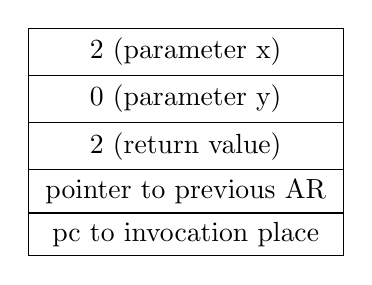
\begin{tikzpicture}
    \node[draw, rectangle split, rectangle split parts=4, 
          minimum width=4cm] at (0,0)
    {
      2  (parameter x) \nodepart{second} 0 (parameter y)
      \nodepart{third} 2 (return value) \nodepart{fourth} pointer to
      previous AR 
    };
    \node[draw, rectangle, minimum width=4cm] at (0,-1.44) 
                                       {pc to invocation place};
  \end{tikzpicture}
\end{enumerate}
}


\newpage

\section{Object-Oriented Programming [15 points]}

\begin{enumerate}
\item Which OO-principle gets easily violated when providing setter
  and getter methods for each field?  \comment{\textbf{1 point}}
\item Let \texttt{Person} be a Smalltalk class defining the following
  methods \texttt{m} and \texttt{n}
\begin{lstlisting}[basicstyle=\small]
Person>>m: aPerson	
  ^aPerson
Person>>n: aPerson	
  ^aPerson
\end{lstlisting}
Consider the following code snippet:
\begin{lstlisting}[basicstyle=\small]
|p1 p2| 
p1:=Person new.
p2:=Person new.
(p1 m: p2) n: nil.       (*a*) 
p1 m: p2; n:nil          (*b*)
\end{lstlisting}
Which objects \lstinline!p1! or \lstinline!p2! are the receivers for the
messages \lstinline!m! and \lstinline!n! in \lstinline!(*a*)! and
\lstinline!(*b*)!?  \comment{\textbf{2 points}}

\item Given the following class
  hierarchy \\
\begin{center}

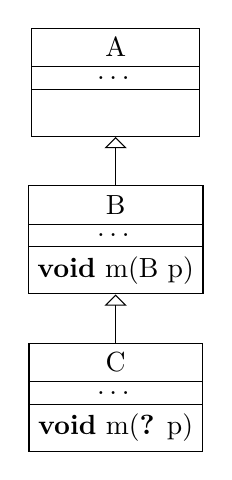
\begin{tikzpicture}
a\node[draw, 
   rectangle split, 
   rectangle split parts=3, 
   minimum width=2cm] (A) at (5,4) 
  {A 
     \nodepart{second} \ldots 
     \nodepart{third} \phantom{\textbf{void} h(A x)}};
\node[draw, 
   rectangle split, 
   rectangle split parts=3, 
   minimum width=2cm] (B) at (5,2) 
  {B 
     \nodepart{second} \ldots 
     \nodepart{third} \textbf{void} m(B p)};
\node[draw, 
   rectangle split, 
   rectangle split parts=3, 
   minimum width=2cm] (C) at (5,0) 
  {C 
    \nodepart{second} \ldots 
    \nodepart{third} \textbf{void} m(\textbf{?} p)};   

\draw[open triangle 90-] (A) -- (B);
\draw[open triangle 90-] (B) -- (C);
\end{tikzpicture}
\end{center}
defining all available classes. 
Give for each of the following overriding semantics (for arguments):
\begin{enumerate}
  \item co-variance,
  \item contra-variance and
  \item invariance
\end{enumerate}
all possible argument types for method \lstinline!m! in class
\lstinline!C! such that \lstinline!m! overrides the method
\lstinline!m! declared in class \lstinline!B!.  \comment{\textbf{3 points}}
\item Which of the overriding
  semantics mentioned in the previous item is \emph{not} safe with
  respect to Liskov's (substitution) principle (if you do not know the
  name give a \emph{short} definition of the semantics you mean)?
  Provide an implementation of the method
\begin{lstlisting}[language=Java, columns=flexible, basicstyle=\small]
void f(A a1, A a2, B b1, B b2, C c1, C c2) { ... }        
\end{lstlisting}
declared in class A consisting of maximal 3 statements exhibiting the
unsafe behavior. \comment{\textbf{2 points}}

\item Consider the following code snippet
\begin{lstlisting}[language=Java, columns=flexible, basicstyle=\small]
void execute(int cmd, Object[] args) {
  if (cmd == CommandIndex.MOV) { 
         // do move with args 
  } else if (cmd == CommandIndex.ADD) {
         // do add with args
  } else if (cmd == CommandIndex.JMP) {
         // do jump with args
  }
}
\end{lstlisting}
which realises a simple interpreter. 
\begin{enumerate}
\item The shown solution is not optimal as adding new commands
  requires to change existing code. Which OO oriented feature allows a
  solution that avoids this problem? \comment{\textbf{1 point}}
\item Describe in \emph{at most} 3 \emph{short} sentences (or draw a
  UML diagram) the OO solution. \comment{\textbf{3 points}}
\end{enumerate}
\item Which of the following statements are true\\
    \begin{tabular}{|p{6cm}|c|c|}\hline
      & True & False \\ \hline
     a) F\# supports classes, but their fields must be immutable & & \\\hline
     b) Mutable variables in F\# are always passed by reference & & \\\hline
     c) One concession of F\#  to the underlying \textsf{.net}
     framework is that types cannot at all be inferred automatically & & \\\hline
     d) F\# supports multiple inheritance of classes & & \\\hline
   \end{tabular}\\
   For your answer draw that table but refer to the statements by a),
   b) etc. instead of writing them again. Wrong answers lead to a
   reduction of points, a negative result does not carry over to other
   sub-assignments. \comment{\textbf{2 points}}
 \item Assume you have two interfaces in F\# named
   \lstinline[language=FSharp]{IPv4} and
   \lstinline[language=FSharp]{IPv6} both declare a method
   \lstinline[language=FSharp]{GetAddress()} which returns the IPv4
   resp.\ IPv6 address. Both kinds of addresses are not compatible. In
   Java this would lead to a problem when a class implements both
   interfaces as no single implementation can cover both
   semantics. Why does F\# not have this kind of problem?  \comment{\textbf{1 point}}
\end{enumerate}

\solution{
  \begin{enumerate}
  \item data encapsulation
  \item (*a*): \texttt{m}: p1 and \texttt{n}: p2\\
    (*b*): \texttt{m}: p1 and \texttt{n}: p1 
  \item \begin{enumerate}
    \item B, C
    \item B, A
    \item B
    \end{enumerate}
  \item co-variance; f(...) { b1.m(b2); }
  \item \begin{enumerate}
    \item dynamic method dispatch
    \item Introduce an (abstract) class \lstinline[language=Java,
      columns=flexible]{Command} declaring an (abstract) method
      \lstinline[language=Java, columns=flexible]{exec(Object[] args)}.
      Subclass the class for each command and implement the body
      accordingly. 
    \end{enumerate}
  \item 
    \begin{tabular}{|p{6cm}|c|c|}\hline
      & True & False \\ \hline
      a) F\# supports classes, but their fields must be immutable & & X \\\hline
      b) Mutable variables in F\# are always passed by reference & & X \\\hline
      c) One concession of F\#  to the underlying \textsf{.net}
      framework is that types cannot be inferred automatically at all &
      & X \\\hline
      d) F\# supports multiple inheritance of classes & & X\\\hline
    \end{tabular}\\
  \item interface methods cannot be called on class types an upcast is
    needed; upcast to different interface types can access idfferent
    methods of same name and signature.
  \end{enumerate}

}

\newpage


\section{Logic Programming [12 points]}

\begin{enumerate}
\item
Given the three clauses
\begin{enumerate}
\item \verb!A || B!
\item \verb!C || D!
\item \verb?!A || D?
\end{enumerate}
state {\em which two} of the clauses can be combined using a resolution step, and give the resulting clause.
\points{1}

\item
For each pair of terms below, state whether the terms can be unified,
and if so, give the variable bindings that result. For example,
\verb!X! and \verb!2! {\em can} be unified, and the result is
\verb!X=2!.
\begin{enumerate}
\item \verb![X|Xs]! and \verb![1,2,3]!
\item \verb![X|Xs]! and \verb![]!
\item \verb!pair(A,y)! and \verb!pair(x,B)!
\item \verb!X! and \verb!Y!
\item \verb!pair(A,A)! and \verb!pair(B,C)!
\item \verb!pair(A,A)! and \verb!pair(b,c)!
\end{enumerate}
\points{3}

\item
Study the following Prolog program:
\begin{verbatim}
father(jack,robert).
father(robert,desmond).
father(robert,william).
mother(catherine,robert).
mother(mary,desmond).
mother(mary,william).
\end{verbatim}
What solutions will Prolog find for the following goals?
\begin{enumerate}
\item \verb!father(X,robert).!
\item \verb!father(robert,X).!
\end{enumerate}
\points{2}

\item
Extend the program above by defining a predicate \verb!parents(X,Y,Z)!
which holds if \verb!X! and \verb!Y! are the parents of \verb!Z!, and
\verb!X! is the father.
\points{1}

\item 
What solutions would Prolog find for the query \verb!parents(X,Y,Z)!?
\points{1}

\item
Study the following Prolog definitions:
\begin{verbatim}
append([],Ys,Ys).
append([X|Xs],Ys,[X|Zs]) :- append(Xs,Ys,Zs).
mystery([],[]).
mystery([X|Xs],Ys) :- mystery(Xs,Zs), append(Zs,[X],Ys).
\end{verbatim}
What solutions will Prolog find for the queries
\begin{enumerate}
\item \verb!mystery([1,2,3],X).!
\item \verb!mystery(X,[1,2,3]).!
\end{enumerate}
\points{2}

\item
One of the \verb!mystery! queries falls into an infinite loop after
printing the solutions. Which one?
\points{1}


\item
Rewrite the definition of \verb!mystery! to find the same solutions,
but so that neither of these queries falls into an infinite loop.
\points{1}

\end{enumerate}


\newpage
\section{Bonus Question on the Guest Lecture [1 point]}

Which application domain was Erlang first developed to address?
\begin{enumerate}
\item Scalable internet services.
\item Telecommunications.
\item Financial services.
\item Databases for cloud computing.
\end{enumerate}
\points{1}

\end{document}
